


\startp
\upar{Магнитное поле} 
Для использующегося зеемановского замедлителя зависимость \cite{vlad} магнитного поля $\sub{B}{exp}$ от координаты $z$ представлена на рис. \ref{fig:zB}. Ось $z$ направлена вдоль ЗЗ, вдоль потока атомов. В соответсвие с \cite{stack} магнитное поле эффективно замедляет атомы, при  $B(z) \propto \sqrt{1-z/z_0}$, на рисунке \ref{fig:zB} видно, что эта зависимость достаточно хорошо приближает $\sub{B}{exp}(z)$.
Параметры аппроксимации: $z_0 = \meas{94}{1}{см}$, $\delta z = \meas{15}{1}{см}$, $B_0 = \meas{740}{13}{Гс}$, $B_1 = \meas{260}{12}{см}$. 

\begin{figure}[ht]
    \centering
    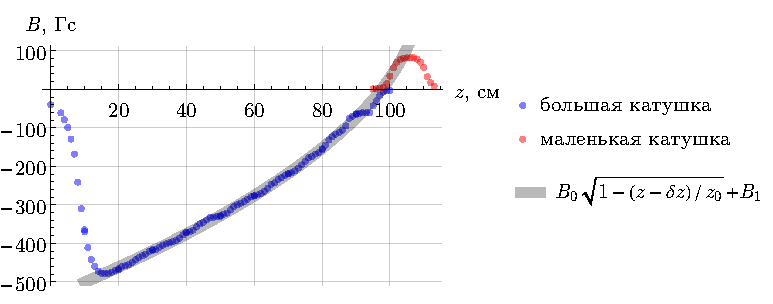
\includegraphics{figs/Bz_v2.pdf}
    \caption{Зависимость магнитного поля внутри зеемановского замедлителя от координаты $z$. Ток маленькой катушки $\sub{I}{small} = 17\,$А, ток большой катушки $\sub{I}{big} = 35\,$А.}
    \label{fig:zB}
\end{figure}

\upar{Тормозящая сила}
Считая, что мы работаем с циклическим переходом на длине волны 410.6 нм, в приближение двухуровневой системы, эффективное сила, действующая со стороны лазерного луча на атом, может быть записана в виде \cite{vlad, suk}
\begin{equation}
    F = \frac{\hbar k \Gamma}{2} \frac{s}{1+s+4({\delta}+k v)^2/\Gamma^2}
    \label{eq:Fbroad}
\end{equation}
где $s=I/\sub{I}{sat}$ -- параметр насыщения, $\sub{I}{sat}$ -- интенсивность насыщения, $v$ -- скорость атома, $k$ -- волновой вектор. 

Уравнение движения запишется в виде
\begin{equation}
    \frac{d v}{d t} = \frac{F}{m},
    \hspace{0.25cm} \overset{v \d t = \d z}{\Leftrightarrow}  \hspace{0.25cm}
    \frac{d v(z)}{d z} = \frac{F(v, z)}{m \, v(z)},
\end{equation}
где $m$ -- масса атома Tm. Таким образом можем найти зависимость $v(z)$ для различных $v_0 \overset{\mathrm{def}}{=} v(z=0)$ (рис. \ref{fig:vZz}а). Характерный вид преобразования распределения атомов по скоростям приведен на рис. \ref{fig:vZz}б для отсройки пучка ЗЗ $\delta = -20\Gamma$, $s=20$, $B(z) \approx \sub{B}{exp}(z)$. 
\begin{figure}[ht]
    \centering
    \subfigure[]{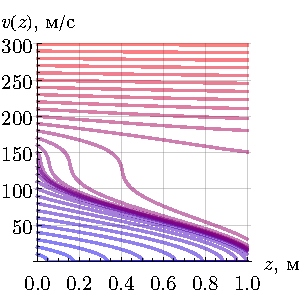
\includegraphics{figs/vz_v2.pdf}}
    \hspace{5 mm} 
    \subfigure[]{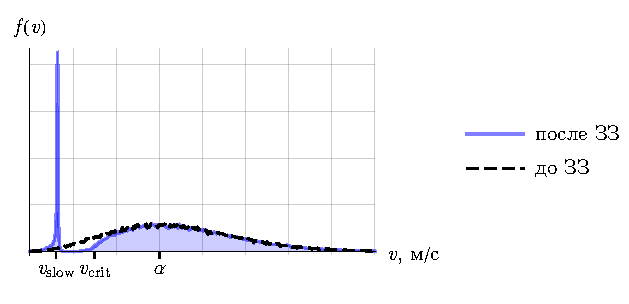
\includegraphics{figs/vdist_v4.pdf}}
    \vspace{-3mm}
    % zeeman_sim_v2
    \caption{a) Зависимость скорости атомов от координаты в зеемановском замедлителе  для различных начальных скоростей $v_0$ при $B_0 = 700\,$Гс, $\delta=-20\Gamma$, $s=20$. б) Характерное преобразование распределения атомов по скоростям после замедления. }
    \label{fig:vZz}
\end{figure}

% заменить график на отнсительные величины

Для атомов со скоростями $v < \sub{v}{crit}$ замедлитель работает эффективно и замедляет до некоторой характерной $\sub{v}{slow}$, рядом с которой в соответствии с \eqref{eq:Fbroad} атомы распределены на масштабе $\frac{1}{2}\Gamma\sqrt{1+s} / k$, характерное преобразование распределения  атомов по скоростям приведено на рис. \ref{fig:vZz}b, полученное в результате моделирования методом Монте-Карло для $10^5$ частиц. Обычно для зеемановского замедлителя выполняется, что $\sub{v}{crit} < \alpha$. 


% ~ 2 м/c * sqrt(1+s)


% \unewpage
\upar{Эффективность замедлителя}
Рассмотрим поток частиц, долетающих до замедлителя с учётом геометрии системы: $v_r/v_z < \sub{\varphi}{in} \sim 1/40$. Частицы распределены в соотвествии с \cite{Lamporesi_2013}
\begin{equation}
    f(v_z, v_r) \propto v_r e^{-(v_r/\alpha)^2} v_z e^{-(v_z/\alpha)^2} \theta(\sub{\varphi}{in} - v_r/v_z).
    \label{ftheta}
\end{equation}
В дальнейшем в моделировании будет использоваться $10^5$ частиц из распределения \eqref{ftheta} для $\alpha = 300\un{м/c}$.

После замедлителя атомы попадают в систему оптическая патока + магнитооптическую ловушка, основным параметром которой является скорость захвата $\sub{v}{cap}$ -- максимальная скорость атома, при которой атом захватывается ловушкой. 


Для оценки эффективности системы ЗЗ + МОЛ введём безразмерный параметр
\begin{equation}
    \eta = \sub{\Phi}{load} / \sub{\Phi}{sol},
    \label{eq:eta}
\end{equation}
равный отношению количества захваченных в МОЛ атомов к количеству атомов, попадающих в замедлитель. Связь $\eta$ с наблюдаемым количеством атомов в МОЛ приведена в \eqref{eq:etaN}. 


Зависимость $\eta(B_0, \sub{v}{cap}, -\delta, s)$ приведена на рисунке \ref{fig:eta}.  Моделирование методом Монте-Карло проводилось для $10^5$ частиц относящихся к распределению в потоке $\sub{\Phi}{sol}$. Учтены конечные размеры пространства внутри замедлителя (трубка радиуса порядка 1 см), влияние гравитации, конечные размеры МОЛ в соответсвии с характерными экспериментальными значениями установки.  В нашем эксперименте характерное значение $\eta \sim 10^{-4} \div 10^{-3}$, c учётом \eqref{phisol}, даёт близкое к экспериментально наблюдаемому значению $\sub{\Phi}{load} = \eta \sub{\Phi}{sol} \sim 10^{8}\,\text{c}^{-1}$. Измерение $\sub{\Phi}{load}$ подробно описаны в разделе \ref{subsec:motload}.

\begin{figure}[ht]
    \centering
    \rotatebox{90}{\hspace{17mm}\scalebox{0.8}{$B_0=700\un{Гс}$ \hspace{38 mm} $B_0=300\un{Гс}$}}
    \hspace{2 mm} 
    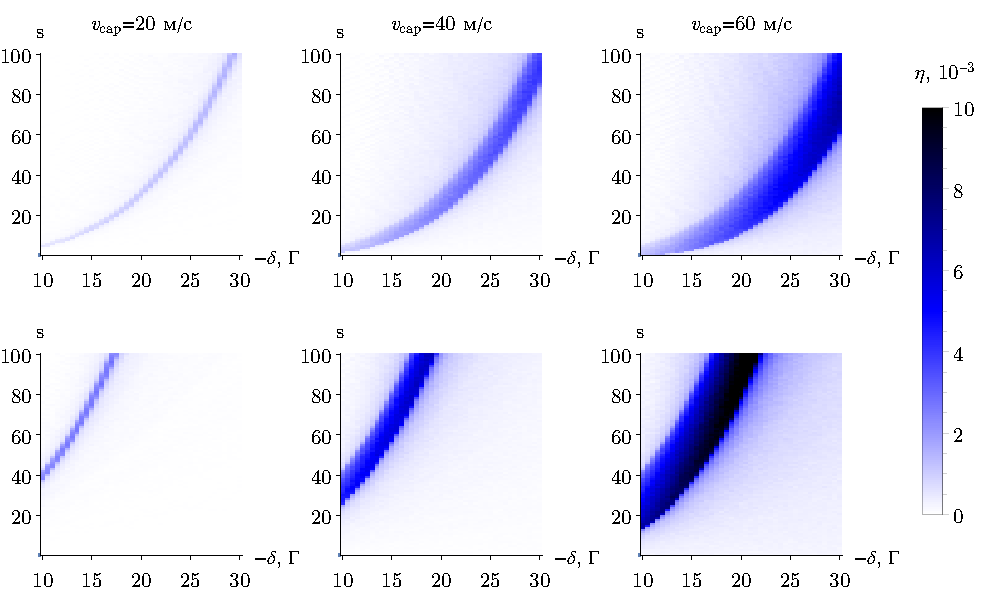
\includegraphics[width=0.95\textwidth]{figs/etas_v4.pdf}
    \caption{Зависимость эффективности работы замедлителя $\eta$ от отстройки луча ЗЗ $\delta$, параметра насыщения $s$ для двух различных значений амплитуды магнитного поля в ЗЗ}
    \label{fig:eta}
\end{figure}


% \red{Здесь анализ картинки, мне не нравится -- переписать.}
% Видно, что есть некоторая оптимальная область параметров (в которой $\sub{v}{slow} < \sub{v}{cap}$), ширина которой увеличивается с увеличением $\sub{v}{cap}$. Формально отстройкой $\delta$ и магнитным полем $B_0$ мы можем увеличивать $\sub{v}{crit}$ \red{(? добавить зависимость $\sub{v}{crit}(B_0, \delta)$, подумать про аналитические оценки)}, ценой увеличения $\sub{v}{slow}$. Увеличением мощности уменьшаем значение $\sub{v}{slow}$ до момента, когда $\sub{v}{slow} < \sub{v}{cap}$. Важно заметить, что зависимость $\eta$ от настраиваемых параметров носит унимодальный характер, что позволяет подбирать оптимальные значения итеративно находя максимум $\eta$ отдельно по каждому из параметров. 


% \phantom{42}

% \textbf{Экспериментальные данные}. \red{Снять зависимость $\NMOT(s)$ для разных магнитных полей.}